\begin{figure}[htbp]
      \centering
    \scriptsize
    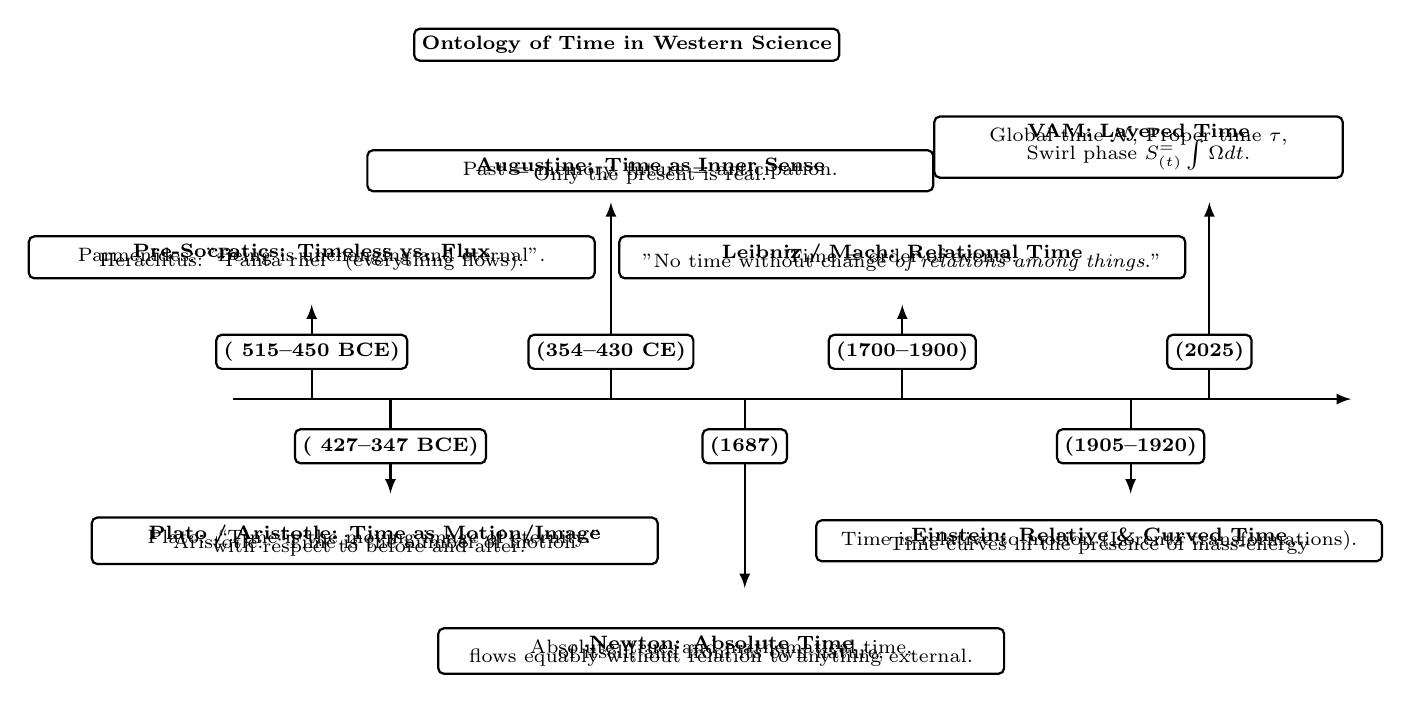
\begin{tikzpicture}[node distance=3.5cm, every node/.style={font=\scriptsize}, >=latex]
    \scriptsize

    % Timeline base
    \draw[->, thick] (-1,0) -- (13.2,0);

    % Arrows above timeline (short, as requested)
    \draw[->, thick] (0,0) -- (0,1.2);       % Pre-Socratics
    \draw[->, thick] (3.8,0) -- (3.8,2.5);   % Augustine
    \draw[->, thick] (7.5,0) -- (7.5,1.2);   % Einstein
    \draw[->, thick] (11.4,0) -- (11.4,2.5); % VAM

    % Arrows below timeline (short, as requested)
    \draw[->, thick] (1.0,0) -- (1.0,-1.2);     % Plato/Aristotle
    \draw[->, thick] (5.5,0) -- (5.5,-2.4);     % Newton
    \draw[->, thick] (10.4,0) -- (10.4,-1.2);     % Leibniz/Mach

        %--- Root title cards (above timeline) ---
    \node[draw, thick, rounded corners=2pt, fill=white, align=center, font=\bfseries ] at (0, .6)   {(~515–450 BCE)};
    \node[draw, thick, rounded corners=2pt, fill=white, align=center, font=\bfseries ] at (3.8, .6) {(354–430 CE)};
    \node[draw, thick, rounded corners=2pt, fill=white, align=center, font=\bfseries ] at (7.5, .6) {(1700--1900)};
    \node[draw, thick, rounded corners=2pt, fill=white, align=center, font=\bfseries ] at (11.4, .6){(2025)};

    %--- Root title cards (below timeline) ---
    \node[draw, thick, rounded corners=2pt, fill=white, align=center, font=\bfseries ] at (1.0,- .6) {(~427–347 BCE)};
    \node[draw, thick, rounded corners=2pt, fill=white, align=center, font=\bfseries ] at (5.5,- .6) {(1687)};
    \node[draw, thick, rounded corners=2pt, fill=white, align=center, font=\bfseries ] at (10.4,- .6) {(1905--1920)};

    % Label
    \node[draw, thick, fill=white, rounded corners=2pt, font=\scriptsize] at (4,4.5) {\textbf{Ontology of Time in Western Science}};

    % Ancient Greek: Parmenides / Heraclitus
    \node[draw, rounded corners=2pt, thick, align=center, fill=white, text width=7cm] at (0,1.8) {
    \textbf{Pre-Socratics: Timeless vs. Flux}  \\[-0.8em]
    Parmenides: "Being is unchanging and eternal".  \\[-0.8em]
    Heraclitus: “Panta rhei” (everything flows).
    };

    % Plato / Aristotle
    \node[draw, rounded corners=2pt, thick, align=center, fill=white, text width=7cm] at (0.8,-1.8) {
    \textbf{Plato / Aristotle: Time as Motion/Image}  \\[-0.8em]
    Plato: “Time is the moving image of eternity.” \\[-0.8em]
    Aristotle: “Time is the number of motion \\[-0.8em]
    with respect to before and after.”
    };

    % Augustine
    \node[draw, rounded corners=2pt, thick, align=center, fill=white, text width=7cm] at (4.3,2.9) {
    \textbf{Augustine: Time as Inner Sense}  \\[-0.8em]
    Past = memory, future = anticipation. \\[-0.8em]
    Only the present is real.
    };

    % Newton
    \node[draw, rounded corners=2pt, thick, align=center, fill=white, text width=7cm] at (5.2,-3.2) {
    \textbf{Newton: Absolute Time}  \\[-0.8em]
    Absolute, true, and mathematical time, \\[-0.8em]
    of itself, and from its own nature, \\[-0.8em]
    flows equably without relation to anything external.
    };


    % Relationalists: Leibniz / Mach
    \node[draw, rounded corners=2pt, thick, align=center, fill=white, text width=7cm] at (7.5,1.8) {
    \textbf{Leibniz / Mach: Relational Time}  \\[-0.8em]
    Time = order of events.  \\[-0.8em]
    "No time without change \textit{of relations among things}."
    };

    % Einstein
    \node[draw, rounded corners=2pt, thick, align=center, fill=white, text width=7cm] at (10.0,-1.8) {
    \textbf{Einstein: Relative \& Curved Time}  \\[-0.8em]
    Time is relative to motion (Lorentz transformations). \\[-0.8em]
    Time curves in the presence of mass-energy
    };


    % VAM
    \node[draw, rounded corners=2pt, thick, align=center, fill=white, text width=5cm] at (10.5,3.2) {
    \textbf{VAM: Layered Time}  \\[-0.8em]
    Global time \( \mathcal{N} \), Proper time \( \tau \),  \\[-0.4em]
    Swirl phase \( S_\text{(t)}^\circlearrowleft = \int \Omega dt \).
    };
    \end{tikzpicture}
    \caption{Historical evolution of temporal ontology: from pre-Socratic polarity to Einstein's spacetime and the layered temporality of the Vortex Æther Model.}
      \label{fig:history-temporal-ontology}
\end{figure}